\documentclass[conference]{IEEEtran}
\title{Mazes vs Pathfinding (algorithms)}
\usepackage{graphicx}
\usepackage{amsmath}
\usepackage{algorithm}
\usepackage[noend]{algpseudocode}
\usepackage{biblatex}
\graphicspath{ {./images/} }
\addbibresource{mazeBib.bib}
\author{Robert A Lane}
\begin{document} 
\maketitle
\begin{abstract}
    \MakeUppercase{read conc after abstract to double check if paper is worth using}


    This paper demonstrates my experiment to run various paathfinding algorithms against
    differeing maze generation algorithms.    
\end{abstract}

\section{Introduction}
This investigation is a 'fun' visual way to compare search algorithms in their speed  accuracy when navigating a variety of mazes generated by different algorithms. This should show some of the strengths and weaknesses of both search and maze algorithms. These maze algorithms are essential creating a spanning tree from the grid. As such we can not only use algrithms that generate trees e.g Binary Tree, but also ones that create minimum spanning trees within the graph.
\section{Literature Review}
might not need
\section{Related work}

what was the paper,defined by the author(surname) -> summarise the paper, bit you need?

\cite{vijayaAnalysisMazeGeneration2024} Vijaya et al discussed the use if mazes within game design. going into how different algorithms can lead to a sense of predictablility and therefore boredom when playing. this particular paper explores depth first search, in both solving the maze as well as generating one - both in the form of recursive backtracking algorithms.

\cite{narendranMazeSolverExploringAlgorithmic2024} Narendran et al explore the effectiveness of various path finding algorithms within a maze. The authors compare fairly basic Breadth-first search, as well as depth-first search with A* search 2 variations aof Markov Decision Process as well as a Enhanced wall follower. The paper goes into depth of how many steps taken, memory usage and time complexity of these algorithhms. This study is particularly relevant as it is very similar to mine. I am differentiating through comparing the first 3 algorithms and last within mazes generated by different algorithms, as well as this these mazes, unlike this work, will not contain loops.

\cite{MazeAlgorithms} James Buck Goes into varying detail about 15 different algorithms to generate mazes. ranging from the fairly standard recursive backtracker, to the wildly inefficient Aldous-Broder algorithm. This blog and his subsequent book \cite{buckMazesProgrammersCode2015a} which goes into more detail about how to implement said algorithms and how they work, whilst also discussing how to add braiding, weaves and different grids.

\cite{} research 4

\cite{} research 5

\cite{} research 6

i think mine is a planning around ai as seraching?? ai arent learning anything

\section{Implementation}
using (git repos autho) repo (reference) we expanded on this to allow for multiple maze algorithms and pathfinders.


\section{The Experiment}
can make a perfect maze without any storage annndd if can garantee the choices(e.g with a seed?) don't even need to store whole maze. Due to the original code the gitRepo I forked off of (reference) there are limitations to the algorithms I have chosen. As such 
\section{The Maze Algorithms}



maze algorithms used will be from Jamis Buck's book Mazes for Programmers\cite{buckMazesProgrammersCode2015a}

section on the maze algorithms/tree/graph gen algorithms I am using
will have subsections
\subsection{binaryTree}

\begin{algorithm}
    \caption{Binary Tree}\label{mazesB}
    \begin{algorithmic}[1]
        \text{boop}
    \end {algorithmic}
\end{algorithm}

\begin{figure}
    \begin{center}
        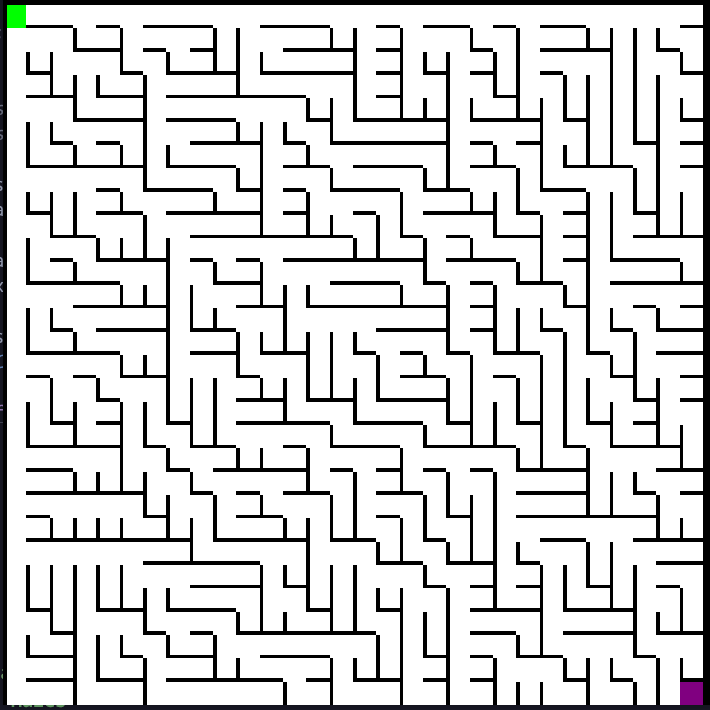
\includegraphics[width=4cm, height = 4cm]{Example_BinaryTree}
        \caption{generation of a binary tree maze given a random seed with a SE bias}\label{fig:BT}
    \end{center}
\end{figure}
A very simple method of generating a maze is by utilising a binary tree. These mazes, however, are extremely biased. A binary tree maze can only pick 2 directions to move to. This creates a visual effect of a diagonal biased depending on the directions you choose % example image of south & east and compare with opposite
the genral upside to this algorithm is that its firstly incredibly simple to implement -> show algorithm <- reference aswell as due to the way it generates can potentially create an infinite maze whilst only storing each cell.
\subsection{depth first/recursive backtracker}
%compare with same seed???

\begin{algorithm}
    \caption{Recursive backtracker}\label{mazesD}
    \begin{algorithmic}[1]
        \text{boop}
    \end {algorithmic}
\end{algorithm}

\begin{figure}
    \begin{center}
        \includegraphics[width = 4cm, height = 4cm]{Example_DepthFirst}
        \caption{Generation of recursive backtracker maze given a random seed}\label{fig:RB}
    \end{center}
\end{figure}
this is a recursive backtracker. The algorithm operates similarly to a depth first search: carving down a branch of a tree all the way till it ends, before looking at the other branches. It then backtracks to the first cell with unvisited neightbours and repeats until there are no unvisited cells. As figure \ref{fig:RB} shows, this results in little to no bias in the generation as appose to a binary tree, see figure \ref{fig:BT}.
%\subsection{Growing Tree algorithm}
\section{The Pathfinding Algorithms}

\subsection{Brepth First}

\subsection{depthFirst}
This is a greedy first algorithm which is essentially the same as the Recursive Backtracker :) only difference instead of creating the maze its solving it. This algorithm can be Modified with a heuristic as so the path picking isn't entirely random.

\subsection{A*}

\subsection{wall Follower}

section on pathfind/tree/graph search algorithms i am using
\MakeUppercase{ USE $\epsilon$-greedy}%wrap in $ to use math
-> with binaryTree due to the bias, compare 'with grain vs against grain'
will have subsections
\section{Results}

\section{Conclusion}

\section{Future Work}


\printbibliography




\end{document}
